% draft for Units specification / update May 2012
%%%%%%%%%%%%%%%%%%%%%%%%%%%%%%%%%%%%%%%%%%%%%%%
%  For an conversion via cgiprint (HTX):
%  See http://vizier.u-strasbg.fr/local/man/cgiprint.htx
\def\ifhtx{\iffalse}    % Lines used only for the HTML version
\ifhtx
% . . .
% . . . Definitions in HTX context
% . . .
\else
\documentclass[12pt,notitlepage,onecolumn]{ivoa}
% . . .
% . . . Definitions in LaTeX context
% . . .
\fi
%%%%%%%%%%%%%%%%%%%%%%%%%%%%%%%%%%%%%%%%%%%%%%%

%% Comment/uncomment lines below to follow your LateX distribution...

\usepackage{natbib} % use author-year citations


\usepackage{prettyref} % ensure consistent cross-references
\newrefformat{sec}{Sect.~\ref{#1}}
\newrefformat{fig}{Fig.~\ref{#1}}
\newrefformat{tab}{Table~\ref{#1}}
\usepackage{varioref}
\newrefformat{tabx}{Table~\vref{#1}}

% Physical units in \rm.  Unstarred version includes leading
% \thinspace.  Starred version doesn't, and is used when referring to
% the unit by itself (eg axis is $B/\units*T$), and is not qualifying
% a number
\makeatletter
\def\units{\@ifstar{\let\un@tsspace\relax    \un@ts}%
                   {\let\un@tsspace\thinspace\un@ts}}
\newcommand{\un@ts}[1]{{\let~\thinspace
  \ifmmode
    \un@tsspace\mathrm{#1}%
  \else
    \nobreak$\un@tsspace\mathrm{#1}$%
  \fi}}

\usepackage{verbatim} % for \verbatiminput
\def\verbatim@font{\fontsize{9}{11}\selectfont\ttfamily}
% \DeclareRobustCommand{\^}{%
%    \ifmmode\nfss@text{\textasciicircum}\else\textasciicircum\fi}
\makeatother

% abbreviation for 'e.g.', which (a) gets spacing right after the full
% stop, and (b) allows us to change the punctuation globally if we
% decide to.
\def\eg{e.g.~}

%%
%% If document is processed with latex, dvips and ps2pdf
%%
\ifx\pdftexversion\undefined
  \usepackage[dvips]{graphicx}
  \DeclareGraphicsExtensions{.eps,.ps}
%% Uncomment following line if you want PDF thumbnails
%  \usepackage[ps2pdf]{thumbpdf}
% for old hyperref, use:
  \usepackage[ps2pdf]{hyperref}
%% for recent hyperref, use:
%  \usepackage[ps2pdf,bookmarks=true,bookmarksnumbered=true,hypertexnames=false,breaklinks=true,%
%  colorlinks,linkcolor=blue,urlcolor=blue]{hyperref}

%%
%% else if document is processed with pdflatex
%%
\else
  \usepackage[pdftex]{graphicx} %% graphics for pdftex (supports .pdf .jpg .png)
  \usepackage{epstopdf}         %% requires epstopdf
%% this is to support .ps files :
  \makeatletter
  \g@addto@macro\Gin@extensions{,.ps}
  \@namedef{Gin@rule@.ps}#1{{pdf}{.pdf}{`ps2pdf #1}}
  \makeatother
%% comment above lines if you have included ps files
%\DeclareGraphicsExtensions{.pdf,.jpg,.png}
%% Uncomment following line if you want PDF thumbnails
%  \usepackage[pdftex]{thumbpdf}
%% for old hyperref, use:
%  \usepackage[ps2pdf]{hyperref}
% for recent hyperref, use:
 \usepackage[pdftex,bookmarks=true,bookmarksnumbered=true,hypertexnames=false,breaklinks=true,%
  colorlinks,linkcolor=blue,urlcolor=blue]{hyperref}
  \pdfadjustspacing=1
\fi
\usepackage[final]{pdfpages}
%\usepackage{tabulary} %%
%%  Header of the document...
%%
% Provide a title for your document
\title{Units in the VO}
% Give date and version number
\date{2012 August 20}

% Choose one document type from below
%\ivoatype{IVOA Note}
%\ivoatype{IVOA Working Draft}
\ivoatype{IVOA Proposed Recommendation}
%\ivoatype{IVOA Recommendation}

\version{1.0}
% Give author list: separate different authors with \\
% You can add email addresses with links \url{mailto:yourname@ivoa.net}
\author{S\'{e}bastien Derri\`ere, Norman Gray, Mireille Louys, \\
Jonathan McDowell, Fran\c{c}ois Ochsenbein, Pedro Osuna, Bruno Rino, \\
Jesus Salgado}
\editor{S\'{e}bastien Derri\`{e}re}

\urlthisversion{\footnotesize{\url{http://www.ivoa.net/Documents/VOUnits/20120820/}}}
\urllastversion{\footnotesize{\url{http://www.ivoa.net/Documents/VOUnits.html}}}
%\previousversion{\footnotesize{\url{http://www.ivoa.net/internal/IVOA/UnitsDesc/WD-VOUnits-v1.0-20120522.pdf}}}
\previousversion{\footnotesize{\url{http://www.ivoa.net/internal/IVOA/UnitsDesc/WD-VOUnits-v1.0-20120718.pdf}}}
%\previousversion{\footnotesize{\url{http://www.ivoa.net/Documents/VOUnits/20120801/}}}



%%%%%%%%%%%%%%%%%
%mir \documentclass[12pt]{article}
%\usepackage{graphicx}
%\usepackage{hyperref}
%\usepackage{psfig}
%\usepackage{html}
%\usepackage{epsf}
%\usepackage{lscape}
%mir \textheight 9.0in \hoffset -0.5in \voffset -0.5in
%\newcommand{\Sensitiv}{Variation}
\newcommand{\Sensitiv}{Sensitivity}
\definecolor{orange}{rgb}{1.0,0.5,0.0}
\newcommand{\unit}[1]{\textbf{\textsf{\color{orange}#1}}}
\usepackage[T1]{fontenc}
\usepackage{longtable}
\usepackage{multirow}
\font\symbo=psyr at 10pt
\def\micro{{\symbo \char109}}

%Mir colors definitions
\newcommand{\bleu}[1]{\textcolor[rgb]{0.00,0.00,1.00}{#1}}
\newcommand{\blue}{\textcolor{blue}}
\newcommand{\violet}{\textcolor[rgb]{0.50,0.00,0.50}}
\newcommand{\brown}{\textcolor[rgb]{0.50,0.10,0.10}}
%%%%%%%%%%%%%%%%%

\begin{document}

\maketitle % print header in standard form
\newpage
\tableofcontents 
\newpage
\section*{Abstract}

This document describes common practices in manipulating
units in astronomical metadata and defines a means of consistent
representation within VO services.

The core of the document contains the recommended rules for writing string representations 
of unit labels, called VOUnits.

\section*{Status of this document}

This is an IVOA Proposed Recommendation made available for public review.
It is appropriate to reference this document only as a recommended standard 
that is under review and which may be changed before it is accepted as a full recommendation.

%This is an IVOA Working Draft for review by IVOA members and
%other interested parties. It is a draft document and may be updated,
%replaced, or rendered obsolete by other documents at any time. It is 
%inappropriate to use IVOA Working Drafts as reference materials or to cite 
%them as other than ``work in progress''.

This document is a substantial update of the previous version 0.2 that
was written within the Data Model IVOA Working Group. As decided in previous
IVOA interoperability meetings, the Semantics working group is now in charge 
of the document. This document is intended to become a full IVOA recommendation,
following agreement within the community and standard IVOA recommendation process.

The place for discussions related to this document is the
Semantics IVOA mailing list {\tt semantics\@@ivoa.net}.

%\def\UrlFont{\small}

A list of current IVOA recommendations and other technical documents can be found at
\url{http://www.ivoa.net/Documents/}.

\section{Introduction}

This document describes the standardised use of Units in the VO
(hereafter simply ``VOUnits''). The introduction gives the motivation for
this proposal in the context of the VO architecture, from the legacy 
metadata available in the resource layer, to the requirements of the various 
VO protocols and standards, to the user layer, including VO applications.

After reviewing and comparing the current practices in the description and usage of units
in \prettyref{sec:current}, \prettyref{sec:proposal} details the proposal for
VOUnits. \prettyref{sec:useCase} lists some use cases and reference implementations.


\subsection{Units in the VO Architecture}

\begin{figure}[htbp]
  \centerline{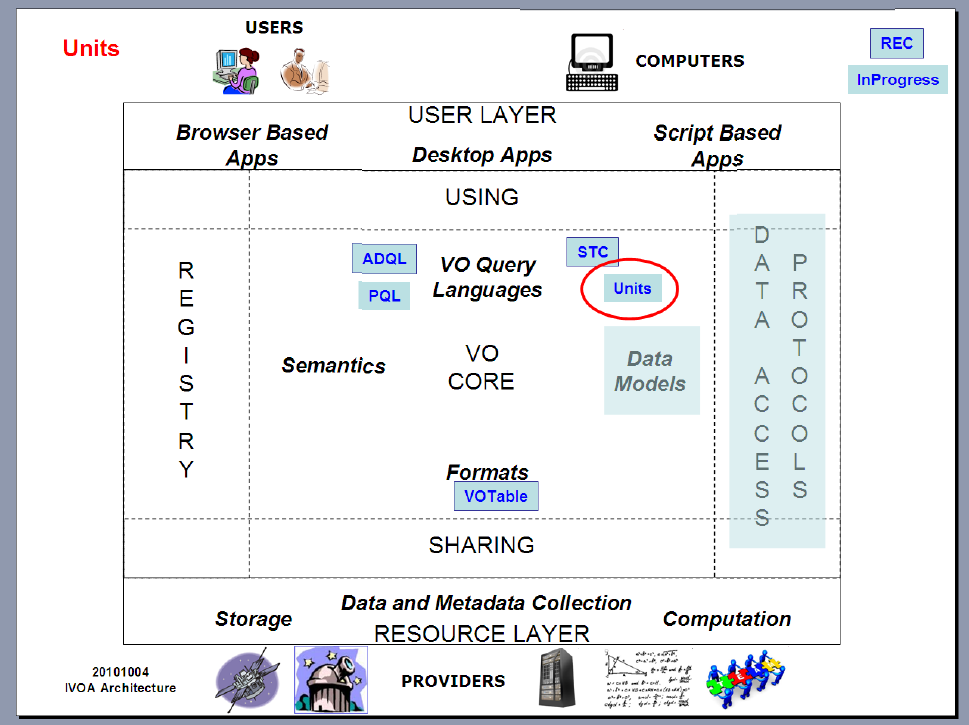
\includegraphics[width=0.9\textwidth]{unitsInIVOA.png}}
  \caption{Units in the VO architecture}
  \label{fig:architecture}
\end{figure}

Generally, every quantity provided in astronomy has a unit attached to
its value or is unitless (\eg a ratio, or a numerical multiplier).  

The Units lie at the core of the VO architecture, as can be seen in \prettyref{fig:architecture}.
Most of the existing data and metadata collections accessible in the resource
layer do have some legacy units, which are mandatory for any scientific use of
the corresponding data.  Units can be embedded in data (\eg FITS headers) or be
implied by convention and/or (preferably) specified in metadata.


Units also appear in the VOTable format \citep{ochsenbein11}, through the use
of a {\tt unit} parameter that can be used in the {\tt FIELD}, {\tt PARAM} and {\tt INFO} 
elements. Because of the widespread dependency of many other VO standards on VOTable,
these standards inherit a dependency on Units.

The Units also appear in many Data Models, through the use of dedicated elements in
the models and schemas.
At present, each VO standard either refers to some external reference document, or 
provides explicit examples of the Units to be used in its scope, on a case-by-case
basis.

The registry records can also contain units, for the description of table metadata.
The definition of VO data protocols uses units by specifying in which units the input
parameters have to be expressed, or by restricting the possible units in which some 
output must be returned.

And last but not least, the tools can interpret units, for example to display
heterogeneous data in a single diagram by applying conversions to a reference 
unit on each axis.

\subsection{Adopted terms and notations\label{sec:notations}}

Discussions about units often suffer from misunderstandings arising from cultural
differences or ambiguities in the adopted vocabulary. For the sake of clarity, in this 
document, the following concepts are used:

\begin{itemize}
\item a {\bf quantity} is the combination of a (numerical) {\em value}, measured for a {\em concept} and expressed in a given {\em unit}. 
In the VO context, the nature of the concept can be expressed with a UCD or a utype. This document does not address the full issue of
representing quantities, but focusses on the {\em unit} part.
\item a {\bf unit} can be expressed in various forms: in natural language (\eg \emph{meters per second squared}), with a combination
of symbols with typographic conventions (\eg \unit{m s$^{-2}$}), or by a simplified text label (\eg \unit{m.s-2}). VOUnit deals with the
label form, which is easier to standardize, parse and exchange. A VOUnit corresponds in the most general case to a combination of
several (possibly prefixed) symbols with mathematical operations expressed in a controlled syntax.
\item a {\bf base unit} is represented by a {\bf base symbol}, with unambiguous meaning.
\item a {\bf prefix} or {\bf scale factor} is prepended to a {\bf base symbol} to scale it by factors of ten.
\item a {\bf symbol} or \unit{sym} is either a base symbol or a prefixed base symbol.
\end{itemize}

Remark: some complex questions, more related to data modeling than to units, such as how a quantity 
is associated to its measurement error, or how groups of coordinates are described, are not addressed in this
document. They can always be broken down, with appropriate modeling, into smaller bits to which VOUnits can
be applied.


\subsection{Purpose of this document}
\label{sec:purpose}

The purpose of this document is to provide a reference specification on how
to write VOUnits, in order to maximize interoperability within the VO. 

VOUnits will not try to reinvent the wheel, and will be as compliant as possible with
legacy metadata in major archives, and astronomers' habits.

By explicitly stating what must (and must not) be used, what may be used, and
giving clear recommendations as to the preferred practices, it should avoid some
common misinterpretations and confusions that are often encountered when dealing with
units.
In particular:
\begin{itemize}
\item We describe (\prettyref{sec:current}) a number of existing unit
  syntaxes, and mention some ambiguities in their
  definition. Application authors should expect to encounter each of
  the syntaxes mentioned in this document (FITS, OGIP and CDS); all of
  these are broadly endorsed by this specification.
\item Where there are some ambiguities in, or contradictions between,
  these specifications, we recommend that application authors should
  resolve them as indicated in this specification.  
% (I'm thinking of the vague words in the FITS spec about whether multiple slashes are permitted)
\item This document defines a syntax, called `VOUnits', which is as
  far as is feasible in the intersection of the three syntaxes, and
  which we recommend that applications should use when writing unit strings.
\end{itemize}

% Data providers are encouraged to follow the VOUnits specifications for expressing
% their metadata. And application developers can rely on these specifications in order
% to know what VOUnits they should expect to face.



\subsection {What this document will not do}
\label{sec:outofscope}

This document is \textbf{not} prescribing what units data providers
employ, nor enforcing that a given quantity be expressed in a
unique way (\eg all distances in \unit{m}).  So long as data are labelled 
in a recognised system, a
translation layer can be provided. Data providers can customise the
translation tools if required. Depending on preference and the
operations required, the user may have a choice of units for their
query and for the result.

VOUnits do not specify how transformation of quantities is done. But VOUnits describe the
units of each quantity in a standard way, allowing to do the conversion if the underlying transformation 
model is known. This is the case for simple operations such as converting light wavelengths into
frequencies, but also for more complex ones such as coordinate conversions or converting
magnitudes into fluxes.

%The former is the domain of the
%PhotometryDataModel to be issued in a separate Data Model effort. See  
%(\violet{\footnotesize{\url{http://www.ivoa.net/cgi-bin/twiki/bin/view/IVOA/PhotometryDataModel}}}) for more information and current developments.\\
%Excellent libraries \eg \textbf{AST} in C \cite{AST}
% (\violet{\footnotesize{\url{http://www.starlink.ac.uk/\~dsb/ast/ast.html}}})\\,
%or \textbf{SLALIB} for Java, already exist for the latter.
%\violet{\footnotesize{\url{http.www.starlink.rl.ac.uk/star/docs/sun67.htx/sun67.html}}}\\

\section{Current use of units}
\label{sec:current}

Many other projects have already produced lists of preferred
representations of units. Those most commonly used in
astronomy are described in this section. 

The four first schemes described below are used as references for the
comparison tables presented later in this document.

\subsection{IAU 1989\label{sec:IAU}}

In the section 5.1 of its Style Manual \citep{wilkins89}, the IAU gives a set
of recommendations for representing units in publications. This document
therefore provides useful reference guidelines, but is not directly
applicable to VOUnits because the recommendations are more intended
for correct typesetting in journals than for standardized metadata exchange.
The IAU style will be summarized in the second column of the comparison tables.

\subsection{OGIP 1993}

NASA has defined a list of character strings specifying the basic physical units 
used within OGIP FITS files \citep{george95}. Rules and guidelines on the construction 
of compound units are also outlined. 

HEASARC datasets follow these conventions, presented in the third column
of the comparison tables.

\subsection{Standards for astronomical catalogues}

The conventions adopted at CDS are summarized in the Standards for Astronomical 
Catalogues, Version 2.0 \citep[\S3.2]{cds00}. They are presented in the fourth column
of the comparison tables.

\subsection{FITS 2010}

Section 4.3 of the reference FITS paper \citep{pence10} describes how unit strings are to be expressed in
FITS files. The recommendations are presented in the fifth column
of the comparison tables.

\subsection{Other usages}

\begin{itemize}
\item
\violet{\footnotesize{\url{http://arxiv.org/pdf/astro-ph/0511616}}}\\ 
Dimensional Analysis applied to spectrum handling in VO context~\citep{osuna05}
offers a mathematical framework to guess and recompute
SI units for any quantity in astronomy.
\item
\violet{\footnotesize{\url{http://www.mel.nist.gov/msid/sima/07_ndml.htm}}}\\
NIST (National Institute of Standards \& Technology) project
UnitsXML builds up an XML representation of units at the granularity
level of a simple symbol string
\item \violet{\footnotesize{\url{https://jsr-275.dev.java.net/}}}\\
JAVA JSR-275 specifies Java packages for the programmatic
handling of physical quantities and their expression as numbers of
units.
\item  \texttt{aips++}
\violet{\footnotesize{\url{http://aips2.nrao.edu/docs/aips++.html}}} and\\
 \texttt{casacore} \violet{\footnotesize{\url{http://code.google.com/p/casacore/}}}\\ contain modules handling units and
quantities with high precision. The packages are mainly in use for
radio astronomy but are designed to be modular and adaptable.  (NB
contrary to the statement on the casacore link, aips++ is still very much in
use as the toolkit behind the {\sc casa} package.)
%\item  IAU SOFA
%\violet{\footnotesize{\url{http://www.iau-sofa.rl.ac.uk/}}} and\\  
%USNO NOVAS
%\violet{\footnotesize{\url{http://aa.usno.navy.mil/software/novas/novas_info.php}}}\\
%implement the IAU 2000 recommendations.
\end{itemize}

\section{Proposal for VOUnits\label{sec:proposal}}

By systematically comparing four reference schemes, the rules for VOUnits are defined in this section.
Various aspects are addressed:
\begin{itemize}
\item how the labels are encoded;
\item what base symbols are allowed and how they are spelled;
\item what prefixes are allowed and how they are used;
\item how symbols are combined.
\end{itemize}

A formal grammar summarizing these conventions is given in \prettyref{sec:vougrammar}.

\subsection{String representation and encoding\label{sec:encoding}}

%    \setlength\LTcapwidth{22cm}
\begin{table}
%\begin{longtable}[th]{|p{0.2\linewidth}|p{0.15\linewidth}|p{0.12\linewidth}|p{0.12\linewidth}|p{0.12\linewidth}|p{0.15\linewidth}|}
  \begin{tabular}{|p{0.2\linewidth}|p{0.15\linewidth}|p{0.1\linewidth}|p{0.1\linewidth}|p{0.15\linewidth}|p{0.15\linewidth}|}
\hline
    & IAU & OGIP  & StdCats & FITS  & VOUnits\\\hline
    Units are strings of chars &  & YES &  & YES & YES\\\hline
    Case sensitive & YES & YES & YES & YES & YES\\\hline
    Character set &  &  & No spaces & ASCII text & ASCII printable\\\hline
\end{tabular}
  \caption{Comparison of string representation and encoding.}
  \label{tab:comparUnitEncoding}
%\end{longtable}
\end{table}

VOUnits must be unit labels suitable for IVOA use (or other electronic manipulation),
and therefore need to be expressed unambiguously in encodings recognised by XML parsers,
Java compilers, etc.  

Following the current usage in unit labels (see \prettyref{tab:comparUnitEncoding}), \emph{VOUnits must be 
case-sensitive strings of chars consisting of printable ASCII characters} (20 to 7E in hexadecimal).

It is therefore not allowed to use special characters such as \AA\ or \micro\ in VOUnits.

\subsection{Base units\label{sec:baseUnits}}

There is a good agreement for the base symbols across the different schemes (see \prettyref{tab:comparUnitBase}).
VOUnits follow the same notations.

For masses, the SI unit is \unit{kg}. However, existing specifications recommend not to use scale factors with
\unit{kg}, but with \unit{g} if needed, which makes the parsing potentially difficult. In VOUnits, only the 
\unit{g} base symbol is defined, and \unit{kg} is implicitly allowed by using the 'k' scale factor with this
base symbol. 

This is just a way to simplify the parsing, by simultaneously allowing scale factors for \unit{g} and
disallowing additional scale factors for \unit{kg}.

No use of the ohm was found in astronomy archives, therefore the possible non-compliance of the OGIP
syntax was not considered critical.
\begin{table}
\begin{tabular}{|p{0.2\linewidth}|p{0.15\linewidth}|p{0.12\linewidth}|p{0.12\linewidth}|p{0.12\linewidth}|p{0.15\linewidth}|}
%\begin{longtable}[th]{|p{0.2\linewidth}|p{0.15\linewidth}|p{0.12\linewidth}|p{0.12\linewidth}|p{0.12\linewidth}|p{0.15\linewidth}|}
\hline
    & IAU & OGIP  & StdCats & FITS  & VOUnits\\\hline
    %\multicolumn{6}{|c|}{Base units} \\\hline
    The 6+1 base SI units\raggedright & \multicolumn{4}{c|}{\unit{m, s, A, K, mol, cd}} & idem \\
     & unit is \unit{kg}, but use \unit{g} with prefixes\raggedright & \unit{kg} & \unit{g} & \unit{kg}, note that \unit{g} is allowed & \unit{g}\\
     %& \multicolumn{4}{c|}{} &  \\
     \hline
    Dimensionless planar and solid angle\raggedright & \multicolumn{4}{c|}{\unit{rad, sr}} & idem \\
    & Use \unit{s}, not sec, for seconds\raggedright &  &  & \unit{deg} preferred for decimal angles & \\\hline
    Derived units with symbols\raggedright & \multicolumn{4}{c|}{\unit{Hz, N, Pa,
      J, W, C, V, S, F, Wb, T, H, lm, lx}} & idem \\
     & \unit{$\Omega$} & \unit{ohm} & \unit{Ohm} & \unit{Ohm} & \unit{Ohm}\\\hline
%     &  &  &  &  & \\\hline
\end{tabular}
  \caption{Comparison of base units.}
  \label{tab:comparUnitBase}
%\end{longtable}
\end{table}

\subsection{Scale factors\label{sec:scaleFactors}}

Following the usage in \prettyref{tab:comparUnitScale}, there are 20 scale factors that can be used as
prefixes to any base symbol (except that~P is not allowed as a scale factor for \unit{a}). One must not use compound prefixes. Prefixes are concatenated to the base
symbol without space, and can not be used without a base symbol.
\begin{table}
\begin{tabular}{|p{0.2\linewidth}|p{0.15\linewidth}|p{0.12\linewidth}|p{0.12\linewidth}|p{0.12\linewidth}|p{0.15\linewidth}|}
%\begin{longtable}[th]{|p{0.2\linewidth}|p{0.15\linewidth}|p{0.12\linewidth}|p{0.12\linewidth}|p{0.12\linewidth}|p{0.15\linewidth}|}
\hline
    & IAU & OGIP & StdCats sec.~3.2.3 & FITS & VOUnits\\\hline
    Scale factors,   & \multicolumn{4}{c|}{\unit{d, c, m, n, p, f, a}} & idem \\
    (multiple) & \multicolumn{4}{c|}{\unit{da, h, k, M, G, T, P, E}}  & \\
    prefixes & \unit{\micro} & \multicolumn{3}{c|}{\unit{u}} & \unit{u}\\
     &  & \multicolumn{3}{c|}{\unit{z, y, Z, Y}} & \unit{z, y, Z, Y}\\\hline
    % & Tab. 5 & Tab. 3 & 3.2.3 & Tab. 5 & \\\hline
    Prefix--symbol concatenation & no space, regarded as single symbol\raggedright & no space, regarded as a single unit string\raggedright & no space & no space (implicit)\raggedright & no space\\\hline
    Prefix-able symbols  & Not \unit{kg}: use \unit{g}\raggedright & All units above, and \unit{eV, pc, Jy, Crab} Only \unit{mCrab} allowed\raggedright & all & all & all (except \unit{P} for \unit{a})\\\hline
    Use compound prefixes & should not & should never & must not & must not & must not\\\hline
\end{tabular}
  \caption{Comparison of scale factors.}
  \label{tab:comparUnitScale}
%\end{longtable}
\end{table}

Remark: the letter \unit{u} is used instead of the \micro\ symbol to represent a factor of $10^{-6}$, 
following the character set defined in \prettyref{sec:encoding}.

\subsection{Astronomy symbols}

The \prettyref{tab:comparUnitAstro} lists symbols used in astronomy to describe times, angles, distances and
a few additional quantities. 

\begin{table}
\begin{tabular}{|p{0.2\linewidth}|p{0.15\linewidth}|p{0.12\linewidth}|p{0.12\linewidth}|p{0.12\linewidth}|p{0.15\linewidth}|}
%\begin{longtable}[th]{|p{0.2\linewidth}|p{0.15\linewidth}|p{0.12\linewidth}|p{0.12\linewidth}|p{0.12\linewidth}|p{0.15\linewidth}|}
\hline
    & IAU & OGIP  & StdCats & FITS  & VOUnits\\\hline
    %\multicolumn{6}{|c|}{Astronomy-related units} \\\hline
    minute & \unit{min, $^\mathrm{m}$} & \unit{min} & \unit{min} & \unit{min} & \unit{min}\\\hline
    hour & \unit{h, $^\mathrm{h}$} & \unit{h} & \unit{h} & \unit{h} & \unit{h}\\\hline
    day & \unit{d, $^\mathrm{d}$} & \unit{d} & \unit{d} & \unit{d} & \unit{d}\\\hline
    year & \unit{a} & \unit{yr} & \unit{a, yr} & \unit{a, yr} Pa (peta a) forbidden& like FITS\\\hline
    arcsecond & \unit{''} & \unit{arcsec} & \unit{arcsec} & \unit{arcsec} & \unit{arcsec}\\\hline
    arcminute & \unit{'} & \unit{arcmin} & \unit{arcmin} & \unit{arcmin} & \unit{arcmin}\\\hline
    degree (angle) & \unit{$^\circ$} & \unit{deg} & \unit{deg} & \unit{deg} & \unit{deg}\\\hline
    milliarcsecond & \unit{mas} (use \unit{nrad}!)\raggedright &  & \unit{mas} & \unit{mas} & \unit{mas}\\\hline
    microarcsec &  &  & \unit{uarcsec} &  & no dedicated symbol, use
    \unit{uarcsec}\\\hline
    cycle & \unit{c, $^\mathrm{c}$} &  &  &  & not used\\\hline
    astronomical unit & \unit{au} & \unit{AU} & \unit{AU} & \unit{AU} & \unit{AU}\\\hline
    parsec & \multicolumn{4}{c|}{\unit{pc}} & \unit{pc}\\\hline
    atomic mass & \unit{u} &  &  & \unit{u} & \unit{u}\\\hline
    electron Volt & \multicolumn{4}{c|}{\unit{eV}} & \unit{eV}\\\hline
    jansky & \multicolumn{4}{c|}{\unit{Jy}} & \unit{Jy}\\\hline
    celsius degree & \unit{$^\circ$C} for meteorology, other use \unit{K}\raggedright&  &  &  & not used\\\hline
    century & ha, cy should not be used &  &  &  & no dedicated symbol, use \unit{ha} or \unit{hyr}\\\hline
\end{tabular}
  \caption{Comparison of astronomy-related units.}
  \label{tab:comparUnitAstro}
%\end{longtable}
\end{table}

Minutes, hours, and days of time must be represented in VOUnits by the symbols \unit{min}, \unit{h} and \unit{d}.
The year can be expressed by \unit{a} (recommended by IAU) or \unit{yr} (common practice), but peta-year must only
be written \unit{Pyr} because \unit{Pa} is the base symbol for pascal.

The astronomical unit must be expressed in upper-case, \unit{AU}, following the legacy practice, and in order to
avoid the (unlikely) confusion with atto-atomic mass.

There are no VOUnit symbols for celsius degrees or century. Temperatures are expressed in kelvin (\unit{K}),
and a century corresponds to \unit{ha} or \unit{hyr}. Note
  that the unit \unit{ha} is \emph{not} hectare, which is the SI
  stipulation~\citep{si-brochure}.\footnote{If large telescope arrays 
    wish to talk of Janskys per hectare, for some reason, they're going
    to have to find some other way of doing so.}


\subsection{Other symbols}

\prettyref{tab:comparUnitDeprecated} corresponds to Table~7 in the IAU document, and the IAU strongly
recommends to no longer use these units. 


\begin{table}
\begin{tabular}{|p{0.2\linewidth}|p{0.15\linewidth}|p{0.12\linewidth}|p{0.12\linewidth}|p{0.12\linewidth}|p{0.15\linewidth}|}
%\begin{longtable}[th]{|p{0.2\linewidth}|p{0.15\linewidth}|p{0.12\linewidth}|p{0.12\linewidth}|p{0.12\linewidth}|p{0.15\linewidth}|}
\hline
    & IAU & OGIP  & StdCats & FITS  & VOUnits\\\hline
    %\multicolumn{6}{|c|}{IAU (Table 7) strongly recommends to no longer use these} \\\hline
    \aa{}ngstr\"om & \unit{\AA} & \unit{angstrom} & 0.1nm & \unit{Angstrom} & \unit{angstrom}, \unit{Angstrom}\\\hline
    micron & \unit{\micro} &  &  &  & not used \\\hline
    fermi & no symbol &  &  &  & not used \\\hline
    barn & \unit{b} & \unit{barn} & \unit{barn} & \unit{barn} & \unit{barn}\\\hline
    cubic centimetre & \unit{cc} &  &  &  & no dedicated symbol\\\hline
    dyne & \unit{dyn} & \unit{} & \unit{} & \unit{} & not used \\\hline
    erg & \unit{erg} & \unit{erg} & No symbol. \unit{mW/m2} used for erg.cm-2.s-1 & \unit{erg} & \unit{erg} \\\hline
    calorie & \unit{cal} & \unit{} & \unit{} & \unit{} & not used \\\hline
    bar & \unit{bar} & \unit{} & \unit{} & \unit{} & not used \\\hline
    atmosphere & \unit{atm} & \unit{} & \unit{} & \unit{} & not used \\\hline
    gal & \unit{Gal} & \unit{} & \unit{} & \unit{} & not used \\\hline
    eotvos & \unit{E} & \unit{} & \unit{} & \unit{} & not used \\\hline
    gauss & \unit{G} & \unit{G} & \unit{} & \unit{G} & \unit{G} \\\hline
    gamma & \unit{$\gamma$} & \unit{} & \unit{} & \unit{} & not used \\\hline
    oersted & \unit{Oe} & \unit{} & \unit{} & \unit{} & not used \\\hline
    Imperial, non-metric & should not be used & \unit{} & \unit{} & \unit{} & not used \\\hline\hline
\end{tabular}
  \caption{Comparison of symbols deprecated by IAU.}
  \label{tab:comparUnitDeprecated}
\end{table}
%\end{longtable}

In order to be compatible with legacy metadata, VOUnit parsers should be able to interpret
symbols for \aa{}ngstr\"om, barn, erg and gauss, as written in the sixth column of \prettyref{tab:comparUnitDeprecated}.
However, data producers are strongly advised to prefer the equivalent notation using symbols and prefixes listed in 
Tables~\ref{tab:comparUnitBase}, \ref{tab:comparUnitScale} and \ref{tab:comparUnitAstro}. 

\prettyref{tab:comparUnitOther} compares other various symbols. The VOUnits symbol
for magnitudes is \unit{mag}.

\begin{table}
\begin{tabular}{|p{0.2\linewidth}|p{0.15\linewidth}|p{0.12\linewidth}|p{0.12\linewidth}|p{0.12\linewidth}|p{0.15\linewidth}|}
%\begin{longtable}[th]{|p{0.2\linewidth}|p{0.15\linewidth}|p{0.12\linewidth}|p{0.12\linewidth}|p{0.12\linewidth}|p{0.15\linewidth}|}
\hline
    & IAU & OGIP  & StdCats & FITS  & VOUnits\\\hline
    magnitude & \multicolumn{4}{c|}{\unit{mag}} & \unit{mag}\\\hline
    rydberg & \unit{} & \unit{} & \unit{Ry} & \unit{Ry} & \multirow{19}{0.15\linewidth}{same as FITS} \\\hline
    solar mass & \unit{$\mathrm{M}_\odot$} &  & \unit{solMass} & \unit{solMass} &\\\cline{1-5}
    solar luminosity & \unit{} & \unit{} & \unit{solLum} & \unit{solLum} &\\\cline{1-5}
    solar radius & \unit{} & \unit{} & \unit{solRad} & \unit{solRad} &\\\cline{1-5}
    light year & \unit{} & \unit{lyr} & \unit{} & \unit{lyr} &\\\cline{1-5}
    count & \unit{} & \unit{count} & \unit{ct} & \unit{ct, count} &\\\cline{1-5}
    photon & \unit{} & \unit{photon} & \unit{} & \unit{photon, ph} &\\\cline{1-5}
    rayleigh & \unit{} & \unit{} & \unit{} & \unit{R} &\\\cline{1-5}
    pixel & \unit{} & \unit{pixel} & \unit{pix} & \unit{pix, pixel} &\\\cline{1-5}
    debye & \unit{} & \unit{} & \unit{D} & \unit{D} &\\\cline{1-5}
    relative to Sun & \unit{} & \unit{} & \unit{Sun} & \unit{Sun} &\\\cline{1-5}
    channel & \unit{} & \unit{chan} & \unit{} & \unit{chan} &\\\cline{1-5}
    bin & \unit{} & \unit{bin} & \unit{} & \unit{bin} &\\\cline{1-5}
    voxel & \unit{} & \unit{voxel} & \unit{} & \unit{voxel} &\\\cline{1-5}
    bit & \unit{} & \unit{} & \unit{bit} & \unit{bit} &\\\cline{1-5}
    byte & \unit{} & \unit{byte} & \unit{byte} & \unit{byte} &\\\cline{1-5}
    adu & \unit{} & \unit{} & \unit{} & \unit{adu} &\\\cline{1-5}
    beam & \unit{} & \unit{} & \unit{} & \unit{beam} &\\\hline
     & \unit{} & \unit{Crab} avoid use & \unit{} & \unit{} & not used \\\hline
    No unit, dimensionless & \unit{} & blank string & \unit{-} & \unit{} & empty string \\\hline
    Unitless in percent & \unit{} &  & \unit{\%} & \unit{} & \unit{} \\\hline
    unknown & \unit{} & \unit{UNKNOWN} & \unit{} & \unit{} & \unit{?} \\\hline
%  \end{tabular}
\end{tabular}
  \caption{Comparison of other symbols.}
  \label{tab:comparUnitOther}
\end{table}
%\end{longtable}

It can be noted that some of the units listed in \prettyref{tab:comparUnitOther} are 
questionable. They arise in fact from a need to describe quantities, when the only
piece of metadata available is the unit label. Count, photon, pixel, bin, voxel, bit,
byte are concepts, just as apple or banana. The associated quantities could be fully
described with a UCD, a value and an void unit label.

It is possible to count a number of bananas, or to express a distance measured in
bananas, but this does not make a banana a reference unit.

The FITS document provides the most general description of all the compared schemes, 
and VOUnits adopts similar definitions, in order to acknowledge at best legacy metadata.
Note that all symbols like \unit{count}, \unit{photon}, \unit{pixel} are always used
in lower case and singular form.

The recommended way to indicate that there is no unit (for example a quantity that
is a character string, or unitless) is to use an empty string rather than blanks
or dashes.


\subsection{Combination of symbols and mathematical expressions}

\prettyref{tab:comparUnitCombine} summarizes how mathematical operations can be applied on
unit symbols for exponentiation, multiplication, division, and other computations.

%\begin{longtable}[th]{|p{0.2\linewidth}|p{0.15\linewidth}|p{0.12\linewidth}|p{0.12\linewidth}|p{0.12\linewidth}|p{0.15\linewidth}|}
%\hline
%    & IAU & OGIP  & StdCats & FITS  & VOUnits\\\hline
%    %\multicolumn{6}{|c|}{Compound units} \\\hline
%    Multiplication & space, except if previous unit ends with superscript; dot (\unit{.}) may be used
%    	& one or more spaces OR one asterix (\unit{*}) with optional spaces on either side 
%	& dot (\unit{.}), no space 
%	& single space OR asterix (\unit{*}, no spaces) OR dot (\unit{.}, no spaces)& \\\hline
%    Division & per. Use negative index or solidus (\unit{/}) 
%    	& slash (\unit{/}) with optional spaces on either side, space not recommended after / OR negative index
%	& \unit{/} with no spaces 
%	& \unit{/} with no spaces 
%	& \\\hline\hline
%    Use of multiple / & MUST never two 
%    	& allowed 
%	& allowed 
%	& may be used, discouraged, math precedence rule & \\\hline\hline
%    \unit{sym} raised to the power $y$ & superscript 
%    	& \unit{sym**($y$)} parenthesis optional if $y>0$ 
%	& nothing: \unit{sym$y$} use +/- sign for \unit{10+21} 
%	& \unit{sym$y$} OR \unit{sym**($y$)} OR \unit{sym\^{}($y$)}, no space & \\\hline\hline
%    Exponential of \unit{sym} &  & \unit{exp(sym)} &  & \unit{exp(sym)} & \\\hline\hline
%    Natural log of \unit{sym} &  & \unit{ln(sym)} &  & \unit{ln(sym)} & \\\hline\hline
%    Decimal log of \unit{sym} &  & \unit{log(sym)} & \unit{[sym]} & \unit{log(sym)} dimensionless argument & \\\hline\hline
%    Square root of \unit{sym} &  & \unit{sqrt(sym)} &  & \unit{sqrt(sym)} & \\\hline\hline
%    Other math &  & {\small \unit{sin(sym), cos(sym), tan(sym), asin(sym), acos(sym), atan(sym), sinh(sym), cosh(sym), tanh(sym)} } &  &  & \\\hline\hline
%    ( ) &  & any allowed & allowed & optional around powers & \\\hline\hline
%    powers & superscripts & decimal and integer fractions allowed & integers only & integer (sign and () optional), OR decimal or ratio between () & \\\hline
%  \caption{Comparison of mathematical expressions and symbols combinations.}
%  \label{tab:comparUnitCombine}
%%\end{table}
%\end{longtable}
\begin{longtable}[th]{|p{0.2\linewidth}|p{0.2\linewidth}|p{0.12\linewidth}|p{0.12\linewidth}|p{0.22\linewidth}|}
\hline
    & IAU & OGIP  & StdCats & FITS \\\hline
    %\multicolumn{6}{|c|}{Compound units} \\\hline
    Multiplication & space, except if previous unit ends with superscript; dot (\unit{.}) may be used\raggedright
    	& one or more spaces OR one asterisk (\unit{*}) with optional spaces on either side\raggedright 
	& dot (\unit{.}), no space 
	& single space OR asterisk (\unit{*}, no spaces) OR dot (\unit{.}, no spaces) \\\hline
    Division & per. Use negative index or solidus (\unit{/})\raggedright
    	& slash (\unit{/}) with optional spaces on either side, space not recommended after / OR negative index\raggedright
	& \unit{/} with no spaces 
	& \unit{/} with no spaces  \\\hline\hline
    Use of multiple / & MUST never use two /\raggedright 
    	& allowed 
	& allowed 
	& may be used, discouraged, math precedence rule \\\hline\hline
    \unit{sym} raised to the power $y$ & superscript 
    	& \unit{sym**($y$)} parenthesis optional if $y>0$ 
	& nothing: \unit{sym$y$} use +/- sign for \unit{10+21} 
	& \unit{sym$y$} OR \unit{sym**($y$)} OR \unit{sym\^{}($y$)}, no space \\\hline\hline
    Exponential of \unit{sym} &  & \unit{exp(sym)} &  & \unit{exp(sym)} \\\hline\hline
    Natural log of \unit{sym} &  & \unit{ln(sym)} &  & \unit{ln(sym)} \\\hline\hline
    Decimal log of \unit{sym} &  & \unit{log(sym)} & \unit{[sym]} & \unit{log(sym)} dimensionless argument \\\hline\hline
    Square root of \unit{sym} &  & \unit{sqrt(sym)} &  & \unit{sqrt(sym)} \\\hline\hline
    Other math &  & {\small \unit{sin(sym), cos(sym), tan(sym), asin(sym), acos(sym), atan(sym), sinh(sym), cosh(sym), tanh(sym)} } &  & not used \\\hline\hline
    ( ) &  & any allowed & allowed & optional around powers \\\hline\hline
    powers & superscripts & decimal and integer fractions allowed & integers only & integer (sign and () optional), OR decimal or ratio between () \\\hline
    Numeric factor & not used & should be avoided; only powers of 10 allowed; should precede any unit string & allowed & optional 10**k, 10\verb|^|k, or 10$\pm$k \\\hline\hline
  \caption{Comparison of mathematical expressions and symbols combinations.}
  \label{tab:comparUnitCombine}
%\end{table}
\end{longtable}

The combination rules is the point where the largest discrepancies between the
different schemes appear. The FITS document summarises the problem of
try to best accomodate the existing schemes:
\label{sec:fitsquote}
\begin{quote}
Two or more base units strings (called str1 and str2 (...)) may be combined using
the restricted set of (explicit or implicit) operators that provide
for multiplication, division, exponentiation, raising arguments
to powers, or taking the logarithm or square-root of an
argument. Note that functions such as log actually require dimensionless
arguments, so that $\log(\unit{Hz})$, for example, actually
means $\log(x/1 \unit{Hz})$. The final units string is the compound
string, or a compound of compounds, preceded by an
optional numeric multiplier of the form \texttt{10**k}, \texttt{10\^{}k}, or \texttt{10$\pm$k}
where~\texttt k is an integer, optionally surrounded by parentheses with
the sign character required in the third form in the absence of 
parentheses. Creators of FITS files are encouraged to use the
numeric multiplier only when the available standard scale factors
(\dots) will not suffice. Parentheses are used for symbol
grouping and are strongly recommended whenever the order
of operations might be subject to misinterpretation. A space
character implies multiplication which can also be conveyed explicitly
with an asterisk or a period. Therefore, although spaces
are allowed as symbol separators, their use is discouraged. Note
that, per IAU convention, case is significant throughout. The IAU
style manual forbids the use of more than one slash (\unit{/}) character
in a units string. However, since normal mathematical precedence
rules apply in this context, more than one slash may be
used but is discouraged.

A unit raised to a power is indicated by the unit string followed,
with no intervening spaces, by the optional symbols \texttt{**}
or \texttt{\^{}} followed by the power given as a numeric expression (\dots). 
The power may be a simple integer, with or
without sign, optionally surrounded by parentheses. It may also
be a decimal number (\eg 1.5, 0.5) or a ratio of two integers
(\eg 7/9), with or without sign, which must be surrounded by
parentheses. Thus meters squared may be indicated by m**(2),
\texttt{m**+2}, \texttt{m+2}, \texttt{m2}, \texttt{m\^{}2}, \texttt{m\^{}(+2)}, etc. and per meter cubed may be
indicated by \texttt{m**-3}, \texttt{m-3}, \texttt{m\^{}(-3)}, \texttt{/m3}, and so forth. Meters to
the three-halves power may be indicated by \texttt{m(1.5)}, \texttt{m\^{}(1.5)},
\texttt{m**(1.5)}, \texttt{m(3/2)}, \texttt{m**(3/2)}, and \texttt{m\^{}(3/2)}, but not by \texttt{m\^{}3/2}
or \texttt{m1.5}.~\cite[\S4.3.1]{pence10}
\end{quote}

This and other ambiguities are discussed in the detailed syntaxes of \prettyref{sec:grammar}.

VOUnits follow the same rules as FITS, as summarized in \prettyref{tab:VOUnitCombine}, and can in
addition be preceded by an arbitrary optional numeric scaling factor (expressed as a floating number with the optional
exponent being expressed as in FITS, with a multiplication symbol).
% XXX Aren't these quantities, rather than units?? 
Examples of valid VOUnits are \unit{2.54cm}, \unit{10+8m}, \unit{3.45 10**(-4)Jy}. 
Scale factors from \prettyref{tab:comparUnitScale} should however be
preferred and used whenever possible.
\emph{Note (NG): these appear to be `quantities' rather than `units',
  in the terminology of \prettyref{sec:notations} -- resolve
  during/after RFC period.}

\begin{table}
\begin{tabular}[bht]{|l|l|}
\unit{str1 str2} & Multiplication \\
\unit{str1*str2} & Multiplication \\
\unit{str1.str2} & Multiplication \\
\unit{str1/str2} & Division \\
\unit{str1**expr} & Raised to the power expr \\
\unit{str1\^{}expr} & Raised to the power expr \\
\unit{str1expr} & Raised to the power expr \\
\unit{log(str1)} & Common Logarithm (to base 10) \\
\unit{ln(str1)} & Natural Logarithm \\
\unit{exp(str1)} & Exponential (e$^\mathrm{str1}$) \\
\unit{sqrt(str1)} & Square root \\
\end{tabular}
 \caption{Combination rules and mathematical expressions for VOUnits.}
  \label{tab:VOUnitCombine}
\end{table}




%\subsection{Quantities}
%\label{sec:quantities}
%
%A quantity, \eg a measurement of a physical value like the speed of
%light, has a value (2.998 10+5), a ucd (phys.veloc), units (km.s-1)
%and is coded using a numerical type (real).
%
%Some quantities are also reused as units. Many units are expressed, or
%converted, in terms of physical constants such as the speed of light,
%\begin{itemize}
%	\item \texttt{$c=$~2.998 10+8~m.s-1;} 
%	\item Boltzman's constant, \texttt{$K_{\mathrm{B}}=$1.38065~10-23}
%	\item \texttt{1 AU $=$ 1.499 10+11 m.}
%\end{itemize}
%
% Many of these are used as units in their own right, \eg  velocities may be expressed as a
%fraction or multiple of c, but c is also used to convert between
%wavelength and frequency, etc. These are combinations of units with
%scaling factors applied, and so can be treated in the same way as any
%other compound unit \eg  the \texttt{Jy} (\texttt{10-26 W.m-2.Hz-1}) .
%
%We need to ensure that we are consistent with the IVOA Quantity model,
%where appropriate.

\subsection{Remarks and good practices}

VOUnits, as described in this document, provide a string serialization of
unit labels compatible with the two principal
means of representation expected in the VO:
\begin{itemize}
\item as an attribute string in a VOTable document: \verb|unit="..."|
\item as a unit element in an XML serialization of some data model: \verb|<unit>...</unit>|
\end{itemize}

Avoiding the use of special characters (\AA, ', ", ...) reduces the
complexity of using VOUnits in query languages or other programmation environments.

Even if enclosing VOUnits with single or double quotes should be sufficient to
facilitate parsing of a general query containing VOUnits, avoiding the use of
white spaces for multiplication should
make the parsing even easier, with the unit label being a single "word", and therefore
the notation in the first line of \prettyref{tab:VOUnitCombine} is discouraged.


Complex data formats are not addressed by VOUnits. While possibly convenient for
humans, sexagesimal coordinates or calendar dates expressed in ISO 8601 are
quantities represented in a complex format, encoded as strings, and as such the
corresponding VOUnit should be an empty string. Expressions such as "d:m:s" or
"ISO 8601" are not valid VOUnits. This should not be a problem, as existing VO 
standards already recommend that coordinates be expressed in decimal degrees.

One can also remark that some quantities like the Modified Julian Date (MJD) are 
not recognized VOUnits. As described in \prettyref{sec:notations}, the quantity MJD can be 
seen as a concept (described by the appropriate UCD or utype), and the corresponding
value will most likely be expressed in days, so the VOUnit will be \unit{d}. There is 
no need in overloading VOUnits to incorporate the description of concepts themselves.

The notion of unit conversion and quantity manipulation is discussed in
\prettyref{sec:conversion}.


\section{Use cases and applications\label{sec:useCase}}

\subsection{Unit parsing}

The rules defined in \prettyref{sec:proposal} allow us to build VOUnit parsers.
Several services can be built on top of a VOUnit parser:

\begin{enumerate}
\item Validation. A service checking that a VOUnit is well written. The output
of such a service can have different levels: fully valid unit; valid syntax, but
not the preferred one (\eg  use of deprecated symbols); parsing error. 
\item Explanation. A service returning a plain-text explanation of the unit label.
\item Typesetting. A service returning an equivalent of the unit label suitable for inclusion in
a \LaTeX\ or HTML document.
\item Dimensional equation. As described by \citet{osuna05}, VOUnits can be translated
into a dimensional equation, allowing to build up conversions methods from one string 
representation to another one (see also \prettyref{sec:conversion}). 
\end{enumerate}

\subsection{Libraries\label{sec:libraries}}

There are a few existing libraries able to interpret unit labels.
In all cases,
some software effort is required if they are to be used in translating
between data provider unit labels, and those to be adopted by
the IVOA for internal use.

One of the most widely-used specialised
astronomical libraries is AST which includes a unit conversion
facility attached to astronomical coordinate systems \citep{berry12}.

Another library has been developed at
CDS\footnote{\url{http://cds.u-strasbg.fr/resources/doku.php?id=units}},
and can be tested online\footnote{\url{http://cdsweb.u-strasbg.fr/cgi-bin/Unit}}. This library covers all
the symbols and notations defined in the standard for astronomical catalogues \citep[\S3.2]{cds00}, as well as
additional symbols and notations.

Recently, Norman Gray started developing
Unity\footnote{\url{https://bitbucket.org/nxg/unity}}, a new
standalone library intended to parse VOUnits, OGIP, StdCats and FITS
formats, and to be used as a vehicle for developing the grammars and
ideas for this present document.  It provides yacc-style grammars for
the various syntaxes, as well as implementing them in parsers written
in Java and~C.  The formal grammar used for VOUnits is given in
\prettyref{sec:vougrammar}.

\subsection{Unit conversion and quantity transformation\label{sec:conversion}}

Unit conversion is the simple task of converting a quantity expressed in a given unit into a different unit, while
the concept remains the same. For example, converting a distance in \unit{pc} in to a distance in \unit{AU} or \unit{km}.
Or converting a flux from \unit{mJy} to \unit{W.m-2.Hz-1}. This is rather easy with existing libraries, using dimensional
analysis or SI units as a reference.

Quantity transformation consists in deriving a new quantity from one or several original
quantities. It is more complex, because it requires to have a precise model 
(a simple equation in simple cases) for computing the transformation. The model involves
quantities, each described with a UCD or utype, value and VOUnit. Some of the quantities
involved might be physical constants (\eg  Boltzmann's constant $k_{\mathrm{B}}$).

Examples of such transformations can be:
\begin{itemize}
\item linear unit conversion: a distance is measured in \unit{pixel} in an image, and needs to be transformed in
the corresponding angular separation in \unit{arcsec}. This can be done if the quantity representing the pixel
scale is given, with its value and a compatible unit like \unit{deg/pixel}.
\item converting a photon wavelength in the corresponding photon energy or frequency.
\item deriving the flux for a given photon emission rate (in \texttt{W}) from Planck's
constant (\texttt{6.63 $10^{-34}$ J.s}), the radiation frequency (in \texttt{GHz}), and the
number of photons emitted per second.
\item transforming a magnitude into a flux, as needed for SED building.
\end{itemize}

VOUnits can help in quantity transformation if all quantities are qualified with proper VOUnits.

\subsection{Query languages}

Including VOUnits in queries is not an easy task. Some guidelines were defined in the
reflexion on ADQL.

\begin{enumerate}
\item All data providers should be encouraged to supply units for each column
of a table. Columns should also have associated UCDs, so that quantities can be
properly identified.

%In most published tables in Astronomical journals and Vizier server as well, unitless values are
%represented by "---". This could be adopted for the VO convention as well.
\item The IVOA needs to provide a parser to relate the native units to the standard IVOA
labels (in this context, the `native units' are the units of the
underlying database table or metadata).   

\item
The default response to a query which does not specify units, will be
in the native units of the table. 
%\emph{We recommand that the output units will be labelled using the IVOA standard label ???}

\item
Where queries involve combining or otherwise operating on the content
of columns to produce an output column with modified units, we can
provide libraries and a parser to assist in assigning and checking a
new unit, and attach this to the returned values via the SQL CAST
operator. 
This is implemented already in database related applications such as Saada, for instance. 
If any column used in responding to a query lacks a necessary unit, the output
involving that column will be unitless.

\item
If the user wants to change the output units with respect to the table
units, this could be done by specifying the units in the initial
SELECT statement. There are several issues to consider: 
	\begin{enumerate}
	\item Does the user also need to include the conversion expression, or does the unit
parser take care of that?  
	\item Can the user use this to assign units (based on prior knowledge) to output from a 
column lacking a unit?
	\end{enumerate}
\end{enumerate} 


\subsection{Broader use in the VO}

\begin{figure}[thb]
  % Requires \usepackage{graphicx}
  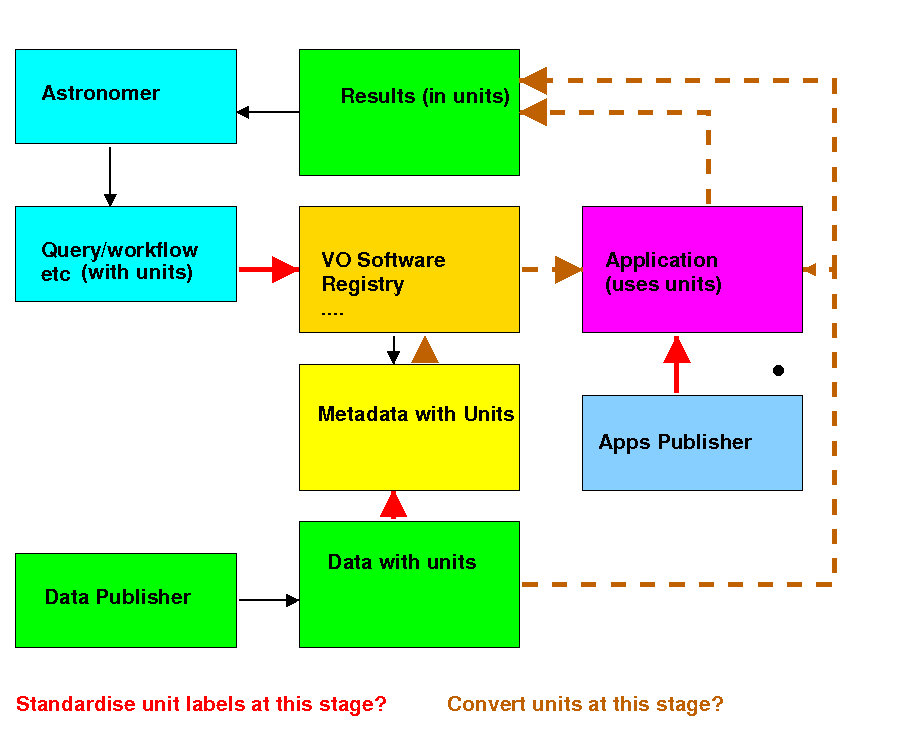
\includegraphics[width=\textwidth]{./units2.jpg}
  \caption{This shows the levels at which conversions might be done.
\textcolor{red}{Thick red arrows}: At the point where an astronomer or
  data provider submits input to the VO, we should provide tools to
  ensure that units are labeled consistently according to VOUnits. 
  This implies that a units parsing step is included prior to metadata ingestion into the VO.
\brown{Dashed brown arrows}: Conversions required to supply results to
  the user in specified or reasonable units \eg  \texttt{J.s-1} to \texttt{W}, are done where and when they are required.}
  \label{fig:units2}
\end{figure}

Different VO entities require and consume metadata with units attached like registries, 
applications and interoperate via protocols. \prettyref{fig:units2} illustrates the places where the IVOA
could intervene to ensure consistent use of units.



\section*{Acknowledgements}

We thank all those participants in IVOA and EuroVO workshops who have
contributed by exposing use cases and providing comments, especially Paddy Leahy, Jeff
Lusted, Arnold Rots, Mark Taylor, Brian Thomas and recent contributors
on the DM forum.
This document is just an update of the previous draft discussed in Strasbourg Interop meeting in 2009.
It will be completed with appropriate grammar and tools to check different levels of consistency for a unit string used in the VO context.


\appendix

\section{Formal grammars\label{sec:grammar}}
% These grammars are extracted from http://bitbucket.org/nxg/unity
% revision f9b7e66b0068

In this section we provide formal (yacc-style) grammars for the four
ASCII-based syntaxes discussed in this document.  The FITS, OGIP and
CDS grammars are not normative: the corresponding specification
documents do not provide grammars, and instead describe the syntaxes
in text, so that the grammars here are deductions from the
specification text.
This unfortunately means that some of these syntaxes are ambiguous.
These ambiguities are discussed in the sections below.  We recommend
that VO applications parse these syntaxes in a way which is consistent
with the grammars here.
%
The grammar for the VOUnits syntax, in \prettyref{sec:vougrammar}, is normative.

We believe that the grammars below are such that if a string 
successfully parses in two distinct grammars, it means the same in
both.

The grammars here are those of the `Unity' package at
\url{https://bitbucket.org/nxg/unity}, which includes lists of
recommended base and derived units in the various syntaxes, plus a
collection of test cases.

In these grammars, the terminals are as given in
\prettyref{tabx:terminals}.
\begin{table}
%\def\={\raggedright\tabularnewline\relax} % avoid problem with \raggedright redefining \\
%\let\=\tabularnewline
\begin{tabular}{rp{9cm}}
\texttt{CARET}&the \texttt{\^{}} character\tabularnewline
\texttt{DIVISION}&the solidus, \texttt{/}\tabularnewline
\texttt{DOT}&the dot/period/full-stop character\tabularnewline
\texttt{FLOAT}&a string matching the regular expression
       \texttt{[-+]?[0-9]+\textbackslash.[0-9]+}\raggedright\tabularnewline
\texttt{OPEN\_P} / \texttt{CLOSE\_P}&parentheses\tabularnewline
\texttt{SIGNED\_INTEGER}&an integer with a required leading sign\raggedright\tabularnewline
\texttt{STAR}&the asterisk\tabularnewline
\texttt{STARSTAR}&a pair of asterisks, \texttt{**}\tabularnewline
\texttt{STRING}&a sequence of letters (a--z and A--Z) plus the percent sign\raggedright\tabularnewline
\texttt{UNSIGNED\_INTEGER}&an integer with no leading sign\raggedright\tabularnewline
\texttt{WHITESPACE}&a non-empty string of space characters (no other whitespace)\raggedright\tabularnewline
\end{tabular}
\caption{\label{tabx:terminals}The terminals used in the grammars}
\end{table}

\subsection{FITS}
\label{sec:fitsgrammar}

For the FITS units syntax, see section~4.3 of~\cite{pence10}, and its
associated tables.  Our preferred FITS grammar is in
\prettyref{tabx:fitsgrammar}.

\begin{table}
\verbatiminput{unity-grammars/unity-fits.txt}
\caption{\label{tabx:fitsgrammar}The FITS grammar}
\end{table}

As noted above in \prettyref{sec:fitsquote}, 
the FITS specification isn't completely clear on the topic of 
solidi, saying `[t]he IAU style manual forbids
the use of more than one solidus (/) character in a units
string. However, since normal mathematical precedence rules apply
in this context, more than one solidus may be used but is
discouraged'.  This does not really resolve the question of whether, for
example, \texttt{kg/m s} should be parsed as \units{kg~m^{-1}~s^{-1}}
or as \units{kg~m^{-1}~s}, since this is a question of both operator
precedence and (left-)associativity, where there might be different
rules internationally, and conflicts between mathematical and
programming-language rules.  Most people would \emph{probably} parse
it as \units{kg~m^{-1}~s^{-1}}, but we trust that most educators would
oblige students to rewrite the expression on the grounds that any
ambiguity is too much.

Here, we resolve the ambiguity by declaring that there can
be only a single expression to the right of the solidus.

It is a consequence of this that nothing can be
successully parsed in two different grammars, with different
meanings.  If the right-hand-side of the division could be a
\texttt{product\_of\_units}, then \texttt{kg /m s} would parse in both
the FITS and OGIP syntaxes,
but mean \units{kg~m^{-1}~s^{-1}} in the FITS syntax, and
\units{kg~m^{-1}~s} in the OGIP one.

Other ambiguities:
\begin{itemize}
\item The FITS spec may or may not be intended to permit 
  \texttt{10+3 /m}, but we don't.
\item It is possible to read the FITS spec as permitting
  \texttt{m\^{}1.5}, without parentheses.  We take it to be
  invalid here.
\end{itemize}
Missing from the grammar is the constraint that the `factor'
\emph{must} be a power of~10 (that is, the \texttt{UNSIGNED\_INTEGER}
must be \texttt{10}).

\subsection{OGIP}
\label{sec:ogipgrammar}

For the OGIP units syntax, see \cite{george95}.  Our preferred OGIP
grammar is in \prettyref{tabx:ogipgrammar}.

\begin{table}
\verbatiminput{unity-grammars/unity-ogip.txt}
\caption{\label{tabx:ogipgrammar}The OGIP grammar}
\end{table}

Specification ambiguities:
\begin{itemize}
\item The OGIP specification permits a space between the leading
  factor and the rest of the unit (by implication from the provided
  examples).
\item OGIP \emph{recommends} having no whitespace after the division
  solidus, but does not forbid it; therefore we permit it in this
  grammar.
\item From its specification text, OGIP appears to permit
  \texttt{str1**y}, where \texttt{y} can be a float, even though none
  of its examples include this.  The same interpretive logic would
  appear to permit \texttt{m**3/2}, but this seems to run too great a
  risk of being misparsed, and we forbid it here.
\item In the same place, the text suggests that \texttt{str1**y} may
  omit the brackets `if~\texttt y is positive', but the context
  suggests that the intention is to permit this if~\texttt y is
  unsigned.  In the grammar here, we permit the omission of the
  brackets only if~\texttt y is unsigned -- that is, \texttt{m**+2},
  like \texttt{m**-2}, is forbidden.
\end{itemize}
Missing from the grammar is the constraint that the `factor'
\emph{must} be a power of~10 (that is, the \texttt{UNSIGNED\_INTEGER}
must be \texttt{10}), and positive.

\subsection{The CDS grammar}
\label{sec:cdsgrammar}

For the CDS units syntax, see \cite[\S3.2]{cds00}.  Our preferred CDS
grammar is in \prettyref{tabx:cdsgrammar}.

\begin{table}
\verbatiminput{unity-grammars/unity-cds.txt}
\caption{\label{tabx:cdsgrammar}The CDS grammar}
\end{table}

The \texttt{CDSFLOAT} terminal is a string matching the regular
expression
\begin{quotation}
\texttt{[0-9]+\textbackslash.[0-9]+x10[-+][0-9]+}
\end{quotation}
(that is, something resembling \texttt{1.5x10+11}).




\subsection{The VOUnits grammar}
\label{sec:vougrammar}

The VOUnits grammar is defined by this section, and the grammar in
\prettyref{tabx:vougrammar}.
This grammar is a strict subset of the
FITS and CDS grammars (in the sense that any VOUnit unit string is a
valid FITS and CDS string, too), and it is almost a subset of the OGIP
grammar, except that it uses the dot for multiplication rather than
star.

\begin{table}
\verbatiminput{unity-grammars/unity-vou.txt}
\caption{\label{tabx:vougrammar}The VOUnits grammar}
\end{table}
As with the other grammars, the `factor'
\emph{must} be a power of~10, and positive.

\clearpage
\section{Updates of this document}
\begin{itemize}
\item 1.0-20120718 to 1.0-20120801
Minor typographical fixes
\item 1.0-20120718 to 1.0-20120801
  \begin{itemize}
    \item Included yacc-style grammars in document.
    \end{itemize}
\item 1.0-20120521 to 1.0-20120718
	\begin{itemize}
	\item Removed external tables refs in tables to avoid confusion.
	\item Removed refs to SOFA and NOVAS.
	\item Precision on the "no unit" case in text.
	\item Added formal grammar in annex.
	\item Minor editing and typo fixes.
	\end{itemize}
\item 1.0-20111216 to 1.0-20120521 
	\begin{itemize}
	\item Typos fixed, removed F. Bonnarel from authors. 
	\item One sentence rephrased in section 1.2 for clarity.
	\item Clarification of \unit{g} and \unit{kg} issue in \prettyref{sec:baseUnits}.
	\item Added remark on \unit{Pa} in \prettyref{sec:scaleFactors}.
	\item Micro-arcsecond and century explained in \prettyref{tab:comparUnitAstro}.
	\item \prettyref{tab:comparUnitDeprecated} completed.
	\item Added numeric factors in \prettyref{tab:comparUnitCombine} and discussion in text.
	\end{itemize}
\item 0.3 to 1.0-20111216 Major rework of the document.
%\item version 0.1 to 0.2
% \begin{itemize}
% \item 20090521
%   \begin{itemize}
%    \item added UCD to Quantity in point 4 of subsection ~\ref{sec:labels}
%    \item added `.' in the notation in unit strings in section ~\ref{sec:simpleuse}
%    \item added a sentence on the help of UCd in quantity in section ~\ref{sec:UML}
%   \end{itemize}
%  \item 20090522
%   \begin{itemize}
%    \item clarified the scope of the model in Section \ref{sec:purpose}
%    \item added references in Section \ref{sec:vocab}
%    \item added requirement to be consistent with Quantity DM in
% Section~\ref{sec:quantities}
%    \item minor clarification and subediting
%   \end{itemize}
% \end{itemize}
\end{itemize}


\bibliographystyle{plainnat-eprints}
\bibliography{bib}


\end{document}
